\chapter{Introducción}
\label{chapter:introduccion}


%%% SECTION
\section{Contexto y justificación del Trabajo}
Cada vez se encuentran más dispositivos conectados entre si no solo en la industria, si no también en los hogares, esta conexión entre dispositivos los hace vulberables a ataques informáticos que pueden afectar en gran medida a los usuarios, no solo pueden provocar un mal funcionamiento de los mismos, si no que también puede provocar la fuga de datos de distinta sensibilidad. La previsión en los futuros años es de cada vez estar más conectados y una pronta detección de los ataques puedo ayudar a evitar los problemas derivados de los mismos, mediante una pronta reacción o frente a la previsión de un ataque.

\vspace{0.5cm}

Actualmente se utilizan distintas medidas de seguridad como control de acceso físico al dispositivo, encriptación de datos, firewalls, securización de red, etc... Sin embargo, en muchos casos la detección de anomalías aplican un umbral estacionario, provocando que en el caso de un ataque ya sea demasiado tarde para reaccionar o no sean capaz de identificar patrones extraños previos al ataque. Con la aplicación de nuevas técnicas se pretende mejorar los tiempos de reacción e incluso predecir cuando puede suceder un ataque.

\section{Explicación de la motivación personal}
La razón principal de la selección del proyecto es la posibilidad de aprender y utilizar técnicas de Machine Learning en un sector desconocido que permita diversificar conocimientos. Cada vez más todo se encuentra conectado e investigar como clasificar cuando se esta produciendo un ataque permite profundizar en conocimientos de seguiridad y aplicarlos en un problema real. 

La aplicación de técnicas en un problema real ayuda a comprender mejor el uso de las herramientas y el por qué y cuando se deben de utilizar. De este modo, se añade un nuevo conocimiento que puede aportar en el ámbito profesional y puede utilizarse también en un entorno privado.


\section{Objetivos del Trabajo}
Los objetivos del trabajo son los siguientes:

\begin{itemize}
  \item Adquisición de conocimiento del sector y de los dispositivos IOT
  \item Lectura y comprensión de las técnicas del estado del arte en detección de anomalías en dispositivos conectados.
  \item Obtención de datos reales de conexiones a dispositivos IOT, en caso de no ser posible, generación de datos sintéticos.
  \item Prueba de las técnicas encontradas y evaluación en el problema actual.
  \item Investigación de algoritmos tradicionales de Machine Learning y su utilidad en el problema actual.
  \item Desarrollo de la solución utilizando los algoritmos más aptos.
  \item Evaluación de la detección de patrones y ataques de las técnicas utilizadas.
  \item Comparar los resultados obtenidos con el estado del arte y probar si existen mejoras frente a los métodos actuales.
\end{itemize}

\section{Descripción general del problema}

En la actualidad, la cantidad de dispositivos informáticos existentes que pueden ser víctimas de un ataques es masiva, por lo que securizar bien los dispositivos es fundamental. A pesar de el uso de distintos protocolos de seguridad, se generan nuevos tipos de ataque todos los días, por lo tanto la detección es una necesidad para evitar los problemas derivados.

\vspace{0.5cm}

La pérdida de control de los dispositivos o la fuga de información de los mismos puede provocar pérdidas millonarias a las empresas o provocar una gran inseguridad a los usuarios de productos IOT, así como provocar posibles daño a infraestructuras o personas. Por otro lado, muchos de los dispositivos pueden no tener la capacidad de computación necesaria para incluir una capa de seguridad robusta, que puede compensarse con una detección temprana. 


\section{Enfoque y método seguido}




\begin{figure}
	\centering
	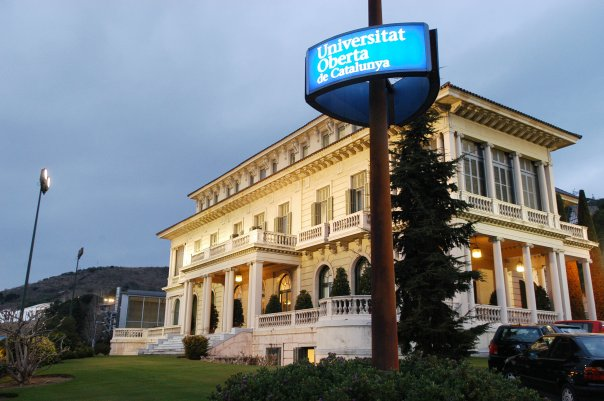
\includegraphics[width=0.6\textwidth]{figs/image1.png}
	\caption{Pie de la imagen.}
	\label{fig:context-anoni1}
\end{figure}

\subsection{Ejemplo de subsection}

Aunque se han realizado importantes avances en preservación de la privacidad en publicación de datos, tales como el modelo \textit{k}-anonymity \cite{Sweeney:2002}.

Un ejemplo de pseudo-código se puede encontrar en el Código \ref{code:RandomSwitch-1}

\begin{algorithm}
	\caption{Pseudocódigo del algoritmo \textit{Random Switch}}
	\label{code:RandomSwitch-1}
	\begin{algorithmic}
		\REQUIRE{El grafo original $G$ y el porcentaje de anonimización $p$ que se desea aplicar.}
		\ENSURE{El grafo $G$ anonimizado.}
		\STATE $num = round(G.num\_edges() * p)$
		\STATE $i = 0$
		\WHILE {$i < num$}
		\STATE {$e_{1} = G.random\_edge()$}
		\STATE $e_{2} = G.random\_edge()$
		\STATE $new\_e_{1} = (e_{1}.origen, e_{2}.origen)$
		\STATE $new\_e_{2} = (e_{1}.destino, e_{2}.destino)$
		\IF {$!G.exist(new\_e_{1})$ \AND $!G.exist(new\_e_{2})$}
		\STATE $G.add\_edge(new\_e_{1})$
		\STATE $G.add\_edge(new\_e_{2})$
		\STATE $G.delete\_edge(e_{1})$
		\STATE $G.delete\_edge(e_{2})$
		\STATE $i=i+1$
		\ENDIF
		\ENDWHILE
		\RETURN $G$
	\end{algorithmic}
\end{algorithm}

Un ejemplo de tabla se puede ver en la Tabla \ref{table:ejemplo_vertex_refi_query}

\begin{table}
	\centering{}
	\begin{tabular}{ l || c | c | l }
		\hline
		Node ID & $\mathcal{H}_{0}$ & $\mathcal{H}_{1}$ & $\mathcal{H}_{2}$ \\
		\hline
		\hline
		Alice & $\epsilon$ & 1 & \{4\}  \\
		\hline
		Bob & $\epsilon$ & 4 & \{1, 1, 4, 4\}  \\
		\hline
		Carol & $\epsilon$ & 1 & \{4\}  \\
		\hline
		Dave & $\epsilon$ & 4 & \{2, 4, 4, 4\}  \\
		\hline
		Ed & $\epsilon$ & 4 & \{2, 4, 4, 4\}  \\
		\hline
		Fred & $\epsilon$ & 2 & \{4, 4\}  \\
		\hline
		Greg & $\epsilon$ & 4 & \{2, 2, 4, 4\}  \\
		\hline
		Harry & $\epsilon$ & 2 & \{4, 4\}  \\
		\hline
	\end{tabular}
	\caption{\textit{Vertex refinement queries}.}
	\label{table:ejemplo_vertex_refi_query}
\end{table}